\section{Theorie}
\label{sec:theorie}
Der Zeeman Effekt beschreibt die Aufspaltung der Spektrallinien eines Atoms
durch ein äußeres magnetisches Feld dadurch, dass sich die Energieniveaus einzelner
Zustände im Magnetfeld verschieben. Dies soll im Folgenden untersucht werden.

\subsection{Quantenzahlen}
\label{subsec:quanten}

Ein gebundenes Elektron in einem Atom kann durch vier Quantenzahlen vollständig beschrieben werden.
Die Hauptquantenzahl $n$ kann ganzzahlige Werte größer als Null annehmen. Sie beschreibt die Schale, auf der sich das Elektron befindet. Die Nebenquantenzahl
$l$ ist charakterisiert die Form des Atomorbitals und kann Werte von $0,1,...,n-1$ annehmen. Die magnetische Quantenzahl des Bahndrehimpulses
$m$ beschreibt die Orientierung des Bahndrehimpulses in $z$-Richtung und liegt zwischen $-l, -l+1,..., l-1, l$.
Die Spinquantenzahl $s$ hat für
Elektronen den Wert $s=\frac{1}{2}$.

\subsection{Magnetisches Moment eines Elektrons}
Jedes Hüllenelektron eines Atoms besitzt einen Bahndrehimpuls $\vec{l}$ und einen
Eigendrehimpuls (Spin) $\vec{s}$. Beide Drehimpulse erzeugen magnetische Momente.
Die Beträge der Impulse folgen aus quantenmechanischen Berechnungen zu
\begin{align}
  |\vec{l}| = \sqrt{l(l+1)} \hbar  \,, \\
  |\vec{s}| = \sqrt{s(s+1)} \hbar \,.
\end{align}
Dabei sind $l$ und $s$ die in Kapitel \ref{subsec:quanten} erläuterten Quantenzahlen und
$\hbar$ ist das reduzierte Planck'sche Wirkungsquantum.
Über das Bohrsche Magneton $\mu_B$
sind die beiden Drehimpulse $\vec{l}$ und $\vec{s}$ mit einem magnetischen Moment
verknüpft. Das Bohrsche Magneton ist definiert als
\begin{equation}
  \mu_B = -\frac{e \hbar}{2 m_e}
\end{equation}
mit der Elementarladung $e$ und der Elektronenmasse $m_e$.
Damit gilt für die magnetischen Momente für die beiden Drehimpulse
\begin{align}
  \vec{\mu_l} = -\mu_B \sqrt{l(l+1)} \vec{l_0} \,, \\
  \vec{\mu_s} = -g_s \mu_B \sqrt{s(s+1)} \vec{s_0} \,.
\end{align}
Dabei ist $g_s$ der sogenannte Landé-Faktor des Elektrons. Dieser beträgt ungefähr 2.

\subsection{Wechselwirkung der magnetischen Momente eines Mehrelektronenatoms}

Die einzelnen magnetischen Momente der Elektronen eines Mehrelektronenatoms können aneinander
koppeln. Im Folgenden werden die $LS$-Kopplung und die $jj$-Kopplung betrachtet.

Die $LS$-Kopplung tritt insbesondere bei Atomen mit niedriger Kernladungszahl auf.
Bei der $LS$-Kopplung ist die Wechselwirkung zwischen den einzelnen Drehimpulsen
$l_i$ der Elektronen sehr groß. Diese addieren sich dann zu einem Gesamtdrehimpuls
$\vec{L}$ der Hülle mit Betrag
\begin{equation}
  |\vec{L}| = \sqrt{L(L+1)} \hbar \,.
\end{equation}
Dabei müssen nur Elektronen in nicht vollständig besetzten Schalen berücksichtigt werden.
Die Werte von $L$ werden in der Atomphysik oft auch mit den Buchstaben $S,P,D,F,...$ gekennzeichnet.
Analog zum Bahndrehimpuls besteht auch der Gesamtspin aus der Summe der einzelnen Spins.
Der Betrag des Gesamtspins ist dann
\begin{equation}
  |\vec{S}| = \sqrt{S(S+1)} \hbar \,.
\end{equation}
Die zughörigen magnetischen Momente sind dann gegeben durch
\begin{align}
  |\vec{\mu_L}| &= \mu_B \sqrt{L(L+1)} \,,\\
  |\vec{\mu_S}| &= g_S \mu_B \sqrt{S(S+1)} \,.
\end{align}
Für nicht zu große Magnetfelder koppeln dann die summierten Drehimpulse $\vec{L}$ und
$\vec{S}$ zum Gesamtdrehimpuls
\begin{equation}
  \vec{J}= \vec{L}+\vec{S}
\end{equation}
mit dem Betrag
\begin{equation}
  |\vec{J}| = \sqrt{J(J+1)}\hbar \,.
\end{equation}

Die $jj$-Kopplung ist bei sehr schweren Atomen dominant. Hier sind die Wechselwirkungen
zwischen den Bahndrehimpulsen und den Spins der einzelnen Elektronen so groß, dass diese
aneinander koppeln. Es gibt dann die Gesamtdrehimpulse
\begin{equation}
  \vec{j_i}=\vec{l_i}+\vec{s_i} \,,
\end{equation}
die dann zum Gesamtdrehiumpuls
\begin{equation}
  \vec{J}= \sum_i \vec{j_i}
\end{equation}
aufaddiert werden können.

\subsection{Aufspaltung der Energieniveaus im homogenen Magnetfeld}

Das gesamte magnetische Moment $\vec{\mu_J}$ der Elektronenhülle setzt sich
zusammen aus dem magnetischen Moment des Bahndrehimpulses $\vec{\mu_L}$ und
dem magnetischen Moment des Spins $\vec{\mu_S}$. Der Betrag des gesamten
magnetischen Moments kann quantenmechanisch zu
\begin{equation}
  |\vec{\mu_J}| = g_J \mu_B \sqrt{J(J+1)}
\end{equation}
bestimmt werden. Dabei ist
\begin{equation}
  g_J = \frac{3J(J+1)-L(L+1)+S(S+1)}{2J(J+1)}
  \label{eqn:lande}
\end{equation}
der Landé-Faktor des Atoms.

In einem äußeren Magnetfeld beobachtet man eine Richtungsquantelung des magnetischen
Moments $\vec{\mu_J}$. Dabei gilt
\begin{equation}
  \mu_{J_z} = -m g_J \mu_B \,,
\end{equation}
wobei $m$ die magnetische Quantenzahl des Bahndrehimpulses ist. Gemäß der in Kapitel
\ref{subsec:quanten} erläuterten Eigenschaften gibt es damit genau $2J+1$ verschiedene
Einstellmöglichkeiten für das magnetische Moment $\vec{\mu_J}$.
Die Energie, die das magnetische Moment im Magnetfeld zusätzlich erhält ist
gegeben durch
\begin{equation}
    E_\text{mag} =-\vec{\mu} \vec{B} = m g_J \mu_B B\,.
\end{equation}
Jede dieser Energien repräsentiert ein Zeeman-Niveau. Ein Zustand mit einer
bestimmten Energie wird also beim Anlegen eines magnetischen Feldes in $2J+1$
Zeeman-Niveaus aufgespalten.
Die Energiedifferenz zwischen zwei aufeinanderfolgenden Zeeman-Niveaus beträgt dabei
\begin{equation}
  \Delta E=g_J \mu_B B\,.
\end{equation}
Die Aufspaltung einer Spektrallinie im magnetischen Feld ist in Abbildung \ref{fig:aufspaltung}
für den Spezialfall $g_J=0$ dargestellt.

\begin{figure}
  \centering
  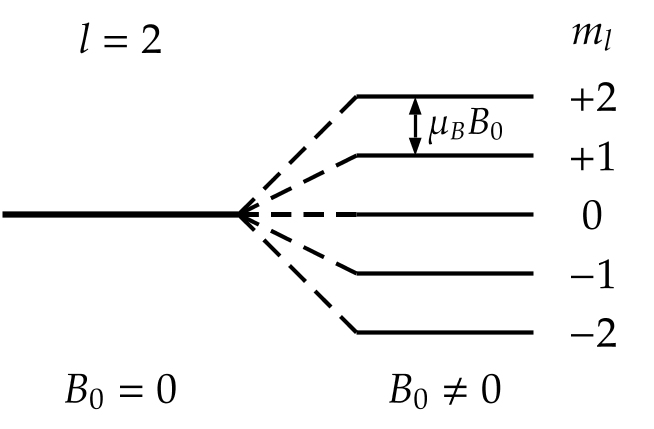
\includegraphics[width=0.7\textwidth]{data/aufspaltung.png}
  \caption{Aufspaltung einer Spektrallinie im magnetischen Feld für den normalen Zeeman-Effekt. Hier gilt
  $g_J=0$. \cite{aufspaltung}}
  \label{fig:aufspaltung}
\end{figure}

\subsection{Optische Übergänge zwischen zeemanaufgespalteten Energieniveaus}

Im Allgemeinen sind optische Übergänge nur dann erlaubt, wenn gilt:
\begin{equation}
  \Delta m= 0, +1 , -1 \,.
\end{equation}
Dabei ist die Strahlung, die mit $\Delta m= 0$ emittiert wird linear in Richtung des
Magnetfeldes polarisiert. Für $\Delta m= \pm1$ ist die Strahlung zirkular polarisiert.
Dabei unterscheiden sich die Drehrichtungen je nach Vorzeichen. Die linear polarisierte
Strahlung wird auch als $\pi$-polarisiert und die zirkular polarisierte Strahlung als
$\sigma$-polarisiert bezeichnet.

Aufgrund dieser Auswahlregeln können nur bestimmte Übergänge zwischen den Zeeman-Niveaus
beobachtet werden. Beim Normalen Zeeman-Effekt, bei dem der Spin nicht berücksichtigt wird
und somit $g_J=1$ gilt,
können drei Gruppen von Spektrallinien beobachtet werden, die jeweils einer der oben
beschriebenen Auswahlregeln entsprechen. Dies ist in Abbildung \ref{fig:cdrot} beispielhaft
für die rote Cadmium Linie dargestellt. Aufgrund der Polarisation der Strahlung kann
die linear polarisierte Komponente jedoch nur bei transversaler Beobachtung gemessen werden.

\begin{figure}
  \centering
  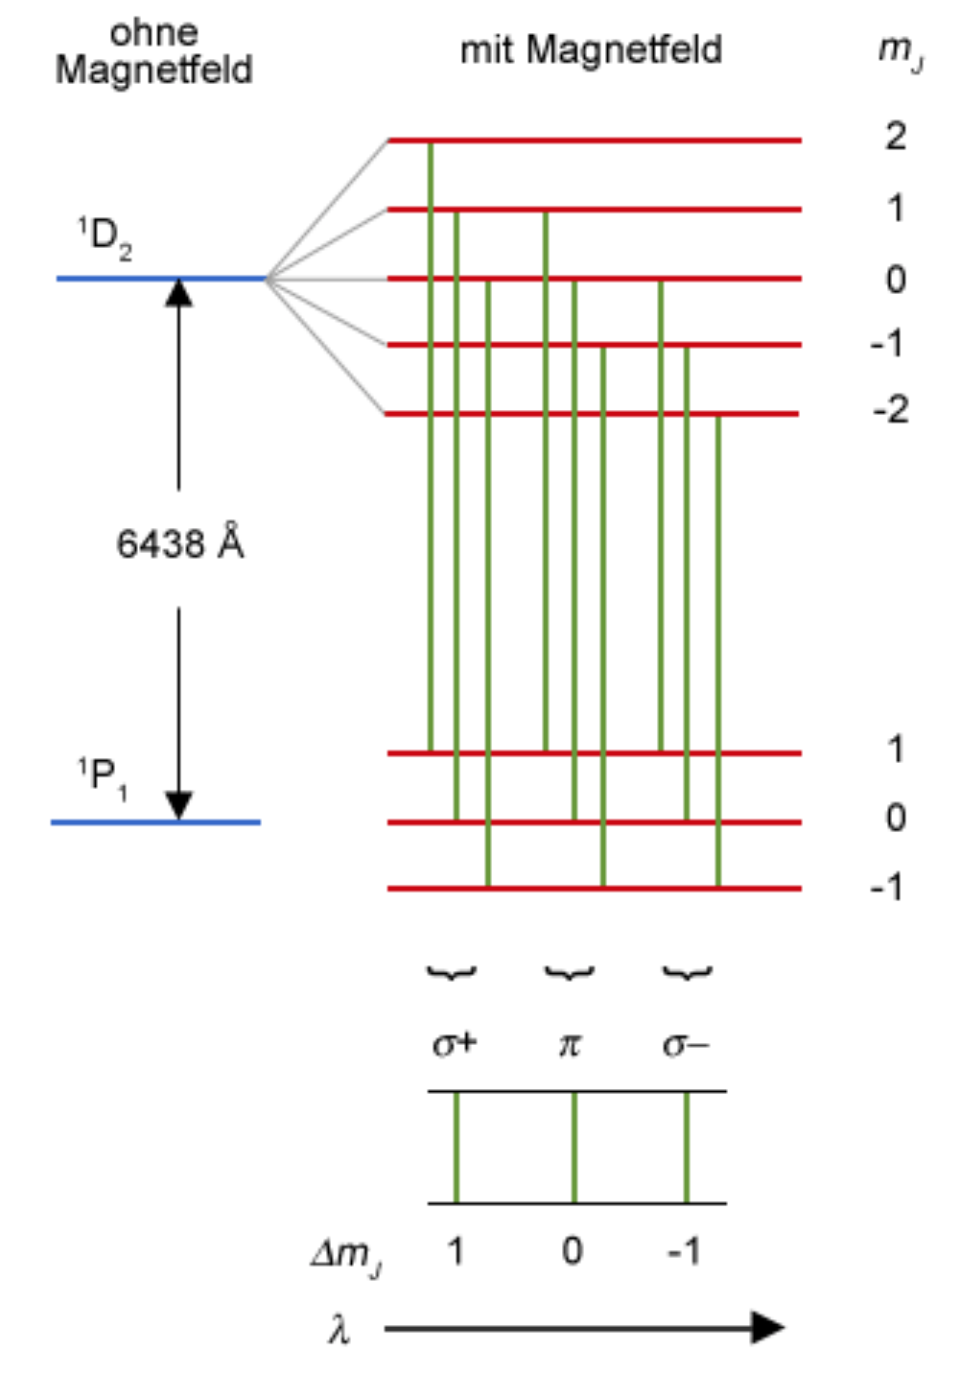
\includegraphics[width=0.5\textwidth]{data/cd_rot.png}
  \caption{Verschiedene Übergänge bei der roten Linie von Cadmium im Magnetfeld. \cite{cdrot}}
  \label{fig:cdrot}
\end{figure}

Beim Anormalen Zeeman-Effekt wird auch der Spin berücksichtigt, woraus folgt, dass
$g_J\neq1$ ist. Die Energie einer Spektrallinie ist hier gegeben durch
\begin{equation}
  \increment E = [m_1 g_J(L_1,S_1,J_1) - m_2 g_J(L_2,S_2,J_2)] \mu_B B +E_0\,,
\end{equation}
wobei die $m_i, L_i, S_i, J_i$ die jeweiligen Quantenzahlen und $E_0$ die Energie bei
ausgeschaltetem Magnetfeld ist. In Abbildung \ref{fig:cdblau} ist beispielhaft der
anormale Zeemaneffekt bei der blauen Cadmium-Linie dargestellt.

\begin{figure}
  \centering
  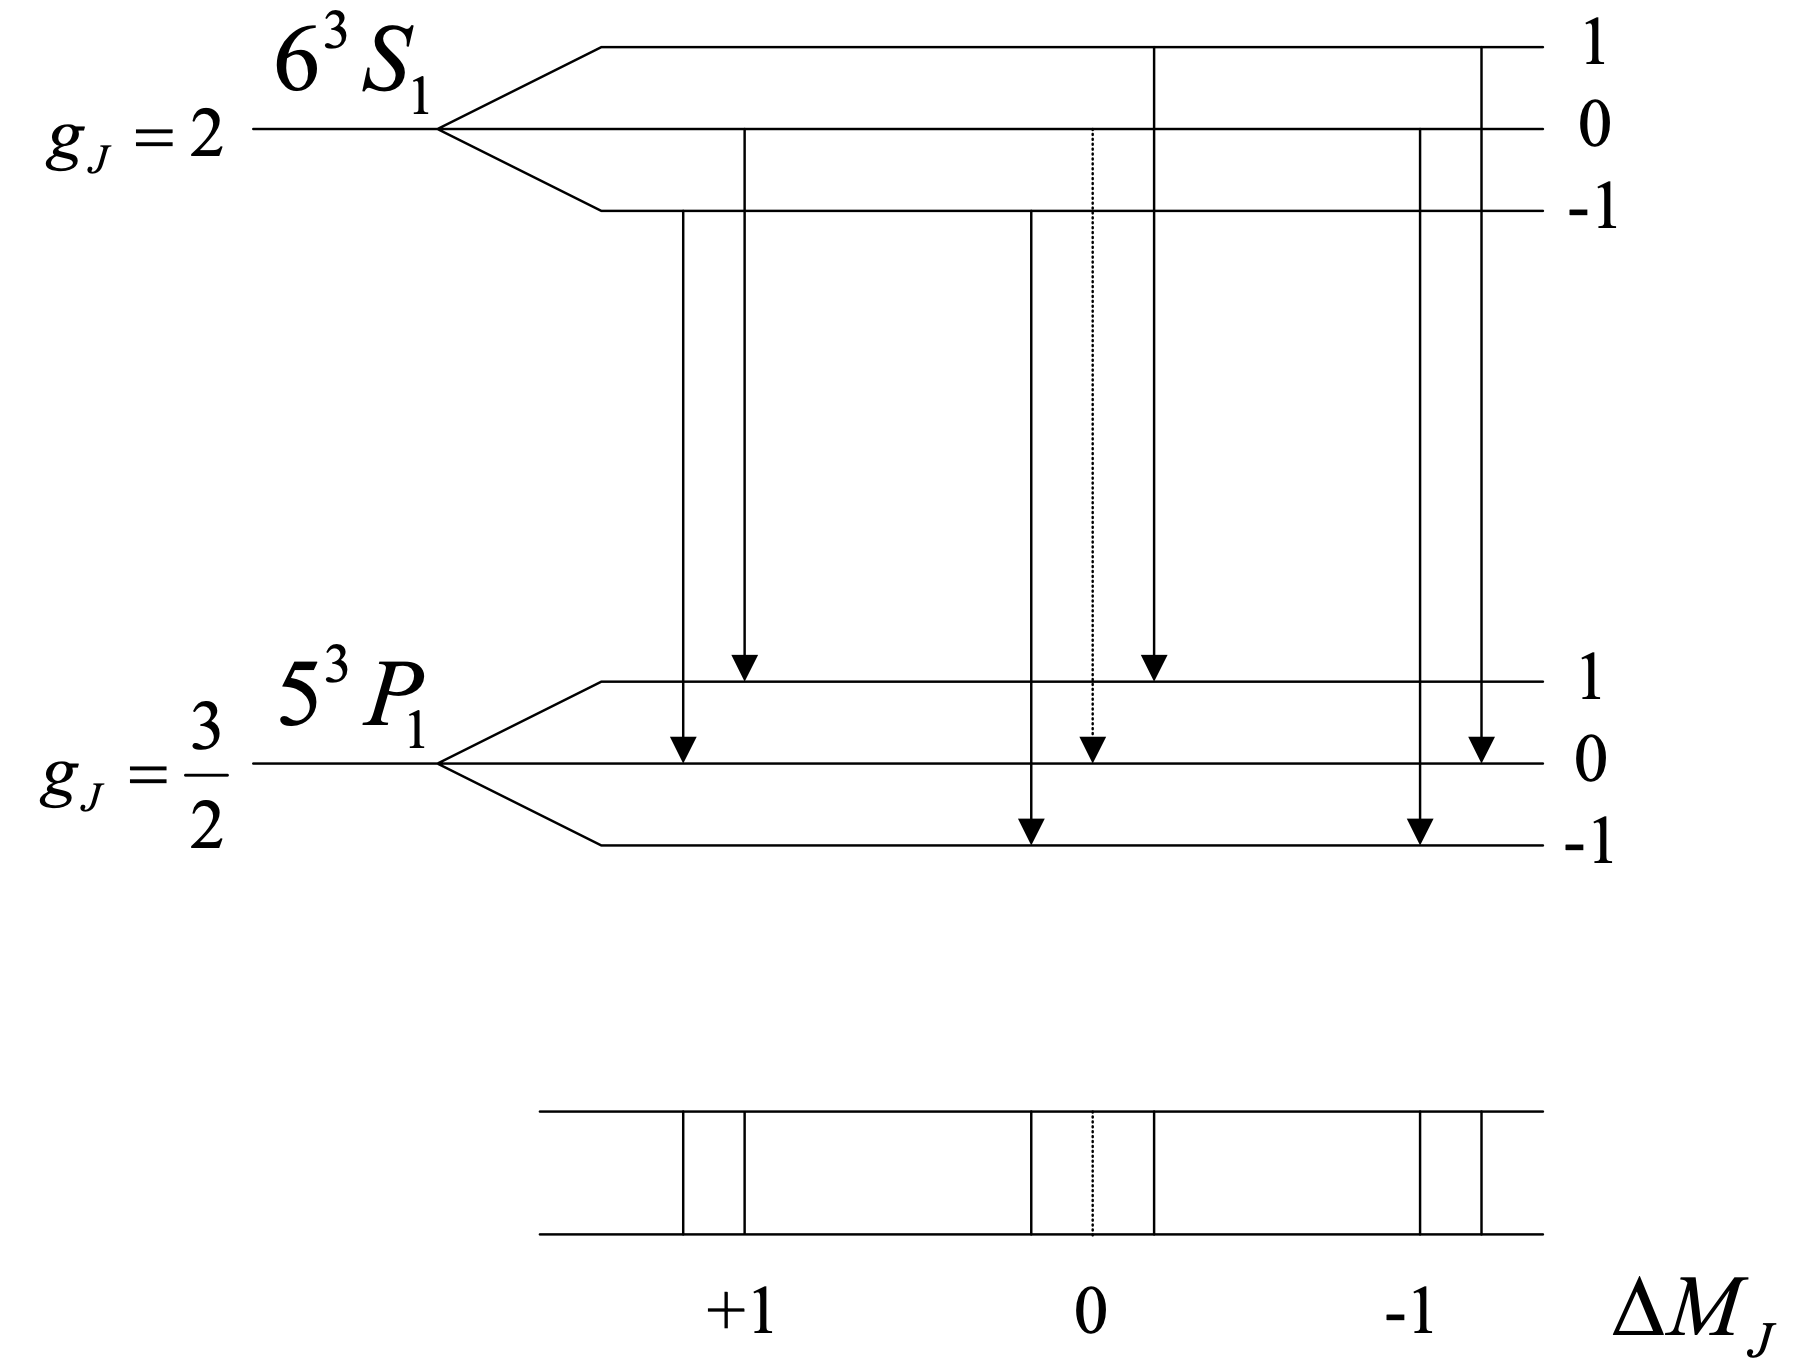
\includegraphics[width=0.5\textwidth]{data/cd_blau.png}
  \caption{Verschiedene Übergänge bei der blauen Linie von Cadmium im Magnetfeld. \cite{cdblau}}
  \label{fig:cdblau}
\end{figure}


\subsection{Optische Übergänge in Cd-Atomen}
\label{subsec:theorieCadmium}

Vorbereitend für die Auswertung werden in diesem Kapitel die Landé-Faktoren für die
zu untersuchenden Spektrallinien berechnet.

Für die rote Spektrallinie mit einer Wellenlänge von $\lambda_0=643{,}8\,$nm wird
der Übergang $\ce{^{1}D_2}$ nach $\ce{^{1}P_1}$ betrachtet. Die Quantenzahlen für
jeden Zustand sind in Tabelle \ref{tab:rot1} dargestellt. Die Energiedifferenzen zwischen
zwei Zeeman-Niveaus bei den verschiedenen Auswahlregeln sind in Tabelle \ref{tab:rot2}
aufgeführt.

\begin{table}
  \centering
  \caption{Quantenzahlen und Landé-Faktor der Energieniveaus der roten Zeeman-Linien.}
  \begin{tabular}{c c c c c c}
    \toprule
    & $L$ & $J$ & $S$ & $m$ & $g_J$ \\
    \midrule
    $\ce{^{1}D_2}$ & 2 & 2 & 0 & -2,-1,0,1,2 & 1 \\
    $\ce{^{1}P_1}$ & 1 & 1 & 0 & -1,0,1, & 1 \\
    \bottomrule
\end{tabular}
  \label{tab:rot1}
\end{table}

\begin{table}
  \centering
  \caption{Energieaufspaltung der roten Zeeman-Linien.}
  \begin{tabular}{c c}
    \toprule
    Übergang & $\increment E$ \\
    \midrule
    $\increment m = -1$ & $-\mu_B B$ \\
    $\increment m = 0$ & 0 \\
    $\increment m = 1$ & $\mu_B B$ \\
    \bottomrule
\end{tabular}
  \label{tab:rot2}
\end{table}

Für die blaue Spektrallinie wird der Übergang $\ce{^{3}P_1}$ nach $\ce{^{3}S_1}$
betrachtet. Die Quantenzahlen für jeden Zustand sind in Tabelle \ref{tab:blau1}
und die Energiedifferenzen für die Übergänge mit den verschiedenen Auswahlregeln
in Tabelle \ref{tab:blau2} aufgeführt.

\begin{table}
  \centering
  \caption{Quantenzahlen und g-Faktor der Energieniveaus der blauen Zeeman-Linien.}
  \begin{tabular}{c c c c c c}
    \toprule
    & $L$ & $J$ & $S$ & $m$ & $g_J$ \\
    \midrule
    $\ce{^{3}P_1}$ & 1 & 1 & 1 & -1, 0, 1 & 1,5 \\
    $\ce{^{3}S_1}$ & 0 & 1 & 1 & -1, 0, 1 & 2 \\
    \bottomrule
\end{tabular}
  \label{tab:blau1}
\end{table}
\begin{table}
  \centering
  \caption{Energienaufspaltung der blauen Zeeman-Linien.}
  \begin{tabular}{c c c}
    \toprule
    Übergang & $m_1 \rightarrow m_2$ & $\increment E$ \\
    \midrule
    $\increment m = -1$ & $1 \rightarrow 0$ & $1{,}5\mu_B B$ \\
    $\increment m = -1$ & $0 \rightarrow -1$ & $2\mu_B B$ \\
    \hline
    $\increment m = 0$ & $1 \rightarrow 1$ & $-0{,}5\mu_B B$ \\
    $\increment m = 0$ & $0 \rightarrow 0$ & 0 \\
    $\increment m = 0$ & $-1 \rightarrow -1$ & $0{,}5\mu_B B$ \\
    \hline
    $\increment m = 1$ & $0 \rightarrow 1$ & $2\mu_B B$ \\
    $\increment m = 1$ & $-1 \rightarrow 0$ & $-1{,}5\mu_B B$ \\
    \bottomrule
    \end{tabular}
  \label{tab:blau2}
\end{table}
In Tabelle \ref{tab:g} sind die theoretischen Vorhersagen für den Wert von $|g|$
aufgeführt.
\begin{table}
  \centering
  \caption{Theoretische Vorhersage für $|g|$.}
  \begin{tabular}{c c c}
    \toprule
    Linie & rot & blau \\
    \midrule
    $\sigma$ & 1 & 1,75 \\
    $\pi$ & 0 & 0,5 \\
    \bottomrule
    \end{tabular}
  \label{tab:g}
\end{table}
